\documentclass{article}


% if you need to pass options to natbib, use, e.g.:
%     \PassOptionsToPackage{numbers, compress}{natbib}
% before loading neurips_2024


% ready for submission
% \usepackage{neurips_2024}


% to compile a preprint version, e.g., for submission to arXiv, add add the
% [preprint] option:
\usepackage[nonatbib, preprint]{neurips_2024}


% to compile a camera-ready version, add the [final] option, e.g.:
% \usepackage[nonatbib, final]{neurips_2024}


% to avoid loading the natbib package, add option nonatbib:
% \usepackage[nonatbib]{neurips_2024}

\usepackage[utf8]{inputenc} % allow utf-8 input
\usepackage[T1]{fontenc}    % use 8-bit T1 fonts
\usepackage{hyperref}       % hyperlinks
\usepackage{url}            % simple URL typesetting
\usepackage{booktabs}       % professional-quality tables
\usepackage{amsfonts}       % blackboard math symbols
\usepackage{nicefrac}       % compact symbols for 1/2, etc.
\usepackage{microtype}      % microtypography
\usepackage{xcolor}         % colors
\usepackage[numbers]{natbib}
\usepackage[ruled]{algorithm2e}
\usepackage{amsmath}
\usepackage{multicol}
\usepackage{tikz}
\usepackage[dvipsnames]{xcolor}
\usepackage{hhline}
\usepackage{booktabs}
\usepackage{float}
\usepackage[title]{appendix}
\graphicspath{{../figures/}}
\definecolor{myblue}{RGB}{74, 144, 226}
\definecolor{myred}{RGB}{255, 2, 27}

\title{Rank Reduction Autoencoders - Enhancing interpolation on nonlinear manifolds.}


% The \author macro works with any number of authors. There are two commands
% used to separate the names and addresses of multiple authors: \And and \AND.
%
% Using \And between authors leaves it to LaTeX to determine where to break the
% lines. Using \AND forces a line break at that point. So, if LaTeX puts 3 of 4
% authors names on the first line, and the last on the second line, try using
% \AND instead of \And before the third author name.
\author{%
  Jad Mounayer\\
  ENSAM Institute of Technology\\
  PIMM, SKF Chair\\
  Blvd de l'Hôpital, Paris \\
  \texttt{jad.mounayer@outlook.com}\\
  % examples of more authors
  \And
  Sebastian Rodriguez\\
  ENSAM Institute of Technology\\
  PIMM, RTE Chair\\
  Blvd de l'Hôpital, Paris\\
  \texttt{sebastian.rodriguez\_iturra@ensam.eu}\\
  \AND
  Chady Ghnatios \\
  ENSAM Institute of Technology\\
  PIMM, SKF Chair\\
  Blvd de l'Hôpital, Paris\\
  \texttt{chady.ghnatios@ensam.eu}\\
  \And
  Charbel Farhat \\
  Department of Aeronautics and Astronautics,\\ Stanford University,\\
  Stanford, 94305,\\
  \texttt{cfarhat@stanford.edu}\\
  \And
  Francisco Chinesta \\
  ENSAM Institute of Technology\\
  PIMM, ESI/Keysight Chair\\
  CNRS@CREATE, Singapore\\
  Blvd de l'Hôpital, Paris\\
  \texttt{francisco.chinesta@ensam.eu} \\
}

\begin{document}


\maketitle


\begin{abstract}
    The efficiency of classical Autoencoders (AEs) is limited in many practical situations. When the latent space is reduced through autoencoders, feature extraction becomes possible. However, overfitting is a common issue, leading to ``holes'' in AEs' interpolation capabilities. On the other hand, increasing the latent dimension results in a better approximation with fewer non-linearly coupled features (e.g., Koopman theory or kPCA), but it doesn't necessarily lead to dimensionality reduction, which makes feature extraction problematic. As a result, interpolating using Autoencoders gets harder. In this work, we introduce the Rank Reduction Autoencoder (RRAE), an autoencoder with an enlarged latent space, which is constrained to have a small pre-specified number of dominant singular values (i.e., low-rank). The latent space of RRAEs is large enough to enable accurate predictions while enabling feature extraction. As a result, the proposed autoencoder features a minimal rank linear latent space. To achieve what's proposed, two formulations are presented, a strong and a weak one, that build a reduced basis accurately representing the latent space. The first formulation consists of a truncated SVD in the latent space, while the second one adds a penalty term to the loss function. We show the efficiency of our formulations by using them for interpolation tasks and comparing the results to other autoencoders on both synthetic data and MNIST.
\end{abstract}

\section{Introduction}\label{sec:intro}
Interpolation of vector functions over a parametric space is an active research topic since accurate interpolation allows the reconstruction of a physical solution in an entire parametric space from a set of pre-computed samples. Multiple techniques have been proposed to perform interpolation, to mention a few, the Proper Orthogonal Decomposition with Interpolation (PODI) \citep{tezzele2019shape, nguyen2022efficient, rama2020towards}, or the sparse-PGD (sPGD) \cite{chinesta2011short}. Most of these techniques are based on Model Order Reductions, such as the Proper Orthogonal Decomposition (POD) \cite{kerschen2005method}, the Proper Generalized Decomposition (PGD) \cite{rodriguez2019non, chinesta2014pgd}, and the Principal Component Analysis (PCA) \cite{gonzalez2018kpca}. These techniques stack the vector functions in what is called the solution matrix, and their efficiency is inversely proportional to the rank of this matrix. If the solution matrix only has a few dominant singular values (i.e., low-rank), it is easier for the aforementioned techniques to reduce the problem and interpolate. However, when this assumption does not apply, they fail to define an efficient surrogate for the correct prediction of physical phenomena. A high-rank solution matrix reduces the efficiency of techniques based on different formulations such as those based on Grassmann manifolds \cite{grasmanian_interp}, the Optimal Transport (OT) \cite{TORREGROSA202212}, or every low-rank technique (e.g. \cite{srebro2003weighted, liu2012robust}).

On the other hand, the nonlinearity in autoencoders with Neural Networks as their encoding and decoding functions makes them appealing to be used as interpolators \cite{NEURIPS2022_interp_manif}. Their modified architectures have been used for different purposes in many applications such as speech recognition \cite{NIPS2014_bilingual}, biophysics \cite{NEURIPS2023_biophysics}, medicine \cite{park2018multimodal}, and others \cite{bank2023autoencoders}. Yet, the efficiency of Vanilla Autoencoders is limited. On one hand, Autoencoders with reduced latent spaces (or Diabolo Autoencoders (DAEs)), can easily overfit the data and are known for having ``holes'' in their latent spaces. On the other hand, even though enlarged latent spaces lead to better approximations with less non-linear behavior (as stated in multiple theories like the Koopman theory or the kPCA), the representations learned are usually of a large dimension which limits both interpolation and feature extraction. This has led to multiple enhancements such as Variational AEs \cite{NIPS2004_VAE, NIPS2017_other_VAE}, Sparse AEs \cite{NIPS2007_sparse}, and denoising AEs \cite{vincent2008extracting} which improved Autoencoders overall but did not definitively solve the interpolation issues.

Neural Networks are increasingly being used for nonlinear reduction techniques \cite{barnett2022neuralnetworkaugmented, NEURIPS2023_kernelSVD}. Recently, the Implicit Rank-Minimizing Autoencoder (IRMAE) \cite{jing2020implicit}, and the Low-Rank Autoencoder (LoRAE) \cite{mazumder2023learning} showcased how increasing the latent space dimension while encouraging a low-rank achieves better results, for both approximation and interpolation. If the latent space is of low rank, the efficiency of all presented interpolation techniques (including basic linear interpolation) in the latent space is enhanced. The resulting Autoencoder would benefit from the large data dimensionality of the latent space to find better approximations while allowing feature extraction because of its low rank. The architecture of IRMAEs consists of adding linear layers between the encoder and the latent space, while LoRAE only adds one linear layer as well as its nuclear norm as a penalty term in the loss. While both papers show how their resulting latent spaces may exhibit a lower rank compared to Vanilla and Variational Autoencoders, their work has some limitations. First, while both architectures may find a low-rank latent space with singular values that are sharply decreasing, they do not enforce the small singular values to go to zero. Accordingly, the decoder always has some noise from the small singular values, even though ideally, we would like to remove their effect entirely. In addition, the computational time of both architectures highly depends on the latent space dimension $L$. Since a long latent space usually helps in achieving better results, both IRMAEs and LoRAEs can be computationally expensive. Finally, both architectures do not provide explicit control over the rank of the latent space. While they include some tuning parameters, we show later in the paper that the optimal parameters proposed in \cite{jing2020implicit, mazumder2023learning} can not reach a satisfying low-rank space.

In this paper, we present the Rank Reduction Autoencoder (RRAE), which has a large latent space restricted to have a low rank. By enforcing the latent space to accept a linear reduction (hence a lower rank), we show that our model resolves the issues previously mentioned. Our architecture includes two proposed formulations: (i) a strong and (ii) a weak one. Throughout the paper, we show that the strong formulation finds orthogonal basis vectors through a principal component analysis of the latent space, while the weak formulation is allowed to find non-orthogonal ones. Further, our results illustrate that both proposed formulations can interpolate efficiently whether between high-rank synthetic solutions, or between MNIST pictures while achieving both a lower latent space rank than the IRMAE and the LoRAE, and a lower computational overhead.

The present paper is structured as follows: Section \ref{sec:HT} presents the architecture and both proposed formulations. Section \ref{sec:insights} explains the insights behind long latent spaces with a low rank on two synthetic examples. Then, we compare the interpolation capabilities of RRAEs with IRMAEs, and LoRAEs on a variety of problems in section \ref{sec:Nuemrical}. We explain the limitations of the proposed formulations in section \ref{sec:limitations}, before finally summarizing the main original contributions of the present paper in section \ref{sec:conclusions}.

\section{Rank Reduction Autoencoders (RRAEs)}\label{sec:HT}
To define the architecture of RRAEs, we begin by defining autoencoder notations. Let $\{X_i\}_{i\in [1, D]} \in \mathbb{R}^T$ be a set of $D$ series of observations, each having $T$ degrees of freedom. We define our input $X\in \mathbb{R}^{T\times D}$ with $X_i$ as its $i$th column. Let, $Y \in \mathbb{R}^{L\times D}$, with $L$, the chosen dimension\footnote[1]{See Appendix \ref{apdx:train} for details on the choice of $L$.} of the latent space. We also define the encoding map $e: \mathbb{R}^{T\times D} \xrightarrow{} \mathbb{R}^{L\times D}$ and the decoding map $d: \mathbb{R}^{L\times D} \xrightarrow{} \mathbb{R}^{T\times D}$. The Vanilla autoencoder can be written as the following two operations,
\begin{equation}
    Y = e(X), \qquad \tilde{X} = d(Y).
\end{equation}
In practice, we usually enforce that the output of the autoencoder gives us back the original data, hence the loss $\mathcal{L}$ usually reads,
\begin{equation}
    \mathcal{L}(X, \tilde{X}) = \Vert X-\Tilde{X}\Vert_2, \quad \text{where,} \quad \Vert \cdot\Vert_2 \text{ is the $L2$-norm}.
\end{equation}
The idea behind RRAEs is to enforce the latent matrix to have a low rank while finding a reduced basis. In other words, if $Y$ has a rank $r$, let $Y = U\Sigma V^T$ be the Singular Value Decomposition (SVD) \cite{stewart1993early, nakatsukasa2017accuracy} of $Y$, with $U\in\mathbb{R}^{L\times r}$, $\Sigma \in\mathbb{R}^{r\times r}$, and $V^T\in\mathbb{R}^{r\times D}$. Let $\{\sigma_i\}_{i \in [1, r]}$ be the sorted diagonal values of $\Sigma$. Thus, by considering the $k$ most significant modes (choice of $k$ discussed in Section \ref{sec:extensions} and Appendix \ref{apdx:train}), it results,
\begin{equation}\label{eqn:trunc}
    Y = \sum_{i=1}^r\sigma_iU_iV_i^T \qquad\Rightarrow\qquad Y\approx \sum_{i=1}^k\sigma_iU_iV_i^T, \qquad k\ll r,
\end{equation}
where $U_i$ is the $i$th column of $U$ and $V_i^T$ is the $i$th row of $V^T$. In other words, we can write $Y_d$, the $d$th column of $Y$ as,
\begin{equation}\label{eqn:alphas}
    Y_d \approx \sum_{i=1}^k\left(\sigma_iU_iV_i^T\right)_d = \sum_{i=1}^k\sigma_iU_iV_{i,d}^T = \sum_{i=1}^k\alpha_{i,d}U_i, \qquad\quad \forall d \in [1, D],
\end{equation}
with $V_{i,d}^T$ being entry $d$ of vector $V_i^T$.

Accordingly, for $k$ modes, each column of $Y$ is defined by $k$ coefficients and $k$ vectors. Further, vectors $U_i$ form a basis for the latent space. We can write \eqref{eqn:alphas} in matrix form as follows,
\begin{equation}\label{eqn:mat_form}
    Y \approx UA, \qquad \text{with: } A_{i,j}=\alpha_{i,j}, \quad U \in \mathbb{R}^{L\times k}. \quad A \in \mathbb{R}^{k\times D},
\end{equation}
Based on \eqref{eqn:alphas}, and \eqref{eqn:mat_form}, we propose two formulations that enforce the low rank of the latent space and find its reduced basis. The architecture is sketched in Figure \ref{fig:mdoel_arch}.
\tikzset{every picture/.style={line width=0.75pt}} %set default line width to 0.75pt 


\begin{figure}



    \tikzset{every picture/.style={line width=0.75pt}} %set default line width to 0.75pt        

    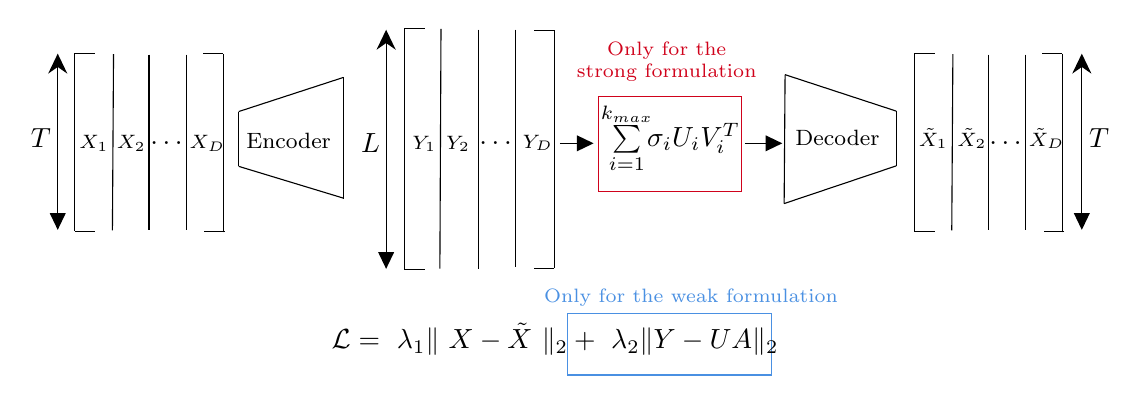
\begin{tikzpicture}[x=0.75pt,y=0.75pt,yscale=-1,xscale=1, scale=0.9]
        %uncomment if require: \path (0,329); %set diagram left start at 0, and has height of 329

        %Straight Lines [id:da21499615368111846] 
        \draw    (37,108.56) -- (37,203.67) ;
        %Straight Lines [id:da16326946357296768] 
        \draw    (37,108.56) -- (47.89,108.56) ;
        %Straight Lines [id:da16265931324232152] 
        \draw    (37,203.67) -- (47.89,203.67) ;
        %Straight Lines [id:da5083389594267504] 
        \draw    (116.56,204.33) -- (116.56,108.67) ;
        %Straight Lines [id:da3615318503641125] 
        \draw    (117.22,203.7) -- (106.33,203.7) ;
        %Straight Lines [id:da9354769223516279] 
        \draw    (116.22,108.6) -- (105.33,108.6) ;
        %Straight Lines [id:da9284204806788381] 
        \draw    (57.67,108.87) -- (57.07,203.27) ;
        %Straight Lines [id:da9687380676381745] 
        \draw    (76.67,109.25) -- (76.67,203.25) ;
        %Straight Lines [id:da30039595434321] 
        \draw    (96.67,109.25) -- (96.67,203.25) ;
        %Straight Lines [id:da782396384119824] 
        \draw    (124.67,139.67) -- (180.67,121.42) ;
        %Straight Lines [id:da9238744798761502] 
        \draw    (124.67,169) -- (180.67,186) ;
        %Straight Lines [id:da44599235940336523] 
        \draw    (180.67,121.42) -- (180.67,186.33) ;
        %Straight Lines [id:da6964885949042201] 
        \draw    (213.3,95.06) -- (213.3,224.17) ;
        %Straight Lines [id:da06959562543054565] 
        \draw    (213.3,95.06) -- (224.19,95.06) ;
        %Straight Lines [id:da030633764479459424] 
        \draw    (213.3,224.17) -- (224.19,224.17) ;
        %Straight Lines [id:da3263511981591738] 
        \draw    (293.52,223.5) -- (293.52,96.17) ;
        %Straight Lines [id:da40502884422960217] 
        \draw    (293.52,223.5) -- (282.63,223.5) ;
        %Straight Lines [id:da8961788198500589] 
        \draw    (293.52,96.3) -- (282.63,96.3) ;
        %Straight Lines [id:da9774520960600939] 
        \draw    (232.97,95.37) -- (232.37,223.77) ;
        %Straight Lines [id:da5075505519042733] 
        \draw    (252.97,95.75) -- (252.97,223.75) ;
        %Straight Lines [id:da21045855349115494] 
        \draw    (272.97,95.75) -- (272.97,222.75) ;
        %Straight Lines [id:da754710144489299] 
        \draw    (124.67,139.67) -- (124.67,169) ;
        %Straight Lines [id:da7099185888654047] 
        \draw    (417.17,119.92) -- (476.67,139.42) ;
        %Straight Lines [id:da66143724081499] 
        \draw    (476.67,168.75) -- (416.67,188.92) ;
        %Straight Lines [id:da31064466545771574] 
        \draw    (417.17,119.92) -- (416.67,188.92) ;
        %Straight Lines [id:da5393972903258972] 
        \draw    (476.67,139.42) -- (476.67,168.75) ;
        %Straight Lines [id:da022156106633165695] 
        \draw    (296.67,156.67) -- (311.67,156.67) ;
        \draw [shift={(314.67,156.67)}, rotate = 180] [fill={rgb, 255:red, 0; green, 0; blue, 0 }  ][line width=0.08]  [draw opacity=0] (8.93,-4.29) -- (0,0) -- (8.93,4.29) -- cycle    ;
        %Straight Lines [id:da38115442380124565] 
        \draw    (395.67,156.67) -- (410.67,156.67) ;
        \draw [shift={(415.67,156.67)}, rotate = 180] [fill={rgb, 255:red, 0; green, 0; blue, 0 }  ][line width=0.08]  [draw opacity=0] (8.93,-4.29) -- (0,0) -- (8.93,4.29) -- cycle    ;
        %Shape: Rectangle [id:dp7709069667907207] 
        \draw  [color={rgb, 255:red, 208; green, 2; blue, 27 }  ,draw opacity=1 ] (317.4,131.47) -- (393.67,131.47) -- (393.67,182.67) -- (317.4,182.67) -- cycle ;
        %Shape: Rectangle [id:dp24666081940562967] 
        \draw  [color={rgb, 255:red, 74; green, 144; blue, 226 }  ,draw opacity=1 ] (300.6,248) -- (409.89,248) -- (409.89,280.67) -- (300.6,280.67) -- cycle ;
        %Straight Lines [id:da9073615867889311] 
        \draw    (27.8,111.67) -- (27.8,200) ;
        \draw [shift={(27.8,203)}, rotate = 270] [fill={rgb, 255:red, 0; green, 0; blue, 0 }  ][line width=0.08]  [draw opacity=0] (8.93,-4.29) -- (0,0) -- (8.93,4.29) -- cycle    ;
        \draw [shift={(27.8,108.67)}, rotate = 90] [fill={rgb, 255:red, 0; green, 0; blue, 0 }  ][line width=0.08]  [draw opacity=0] (10.72,-5.15) -- (0,0) -- (10.72,5.15) -- (7.12,0) -- cycle    ;
        %Straight Lines [id:da1988310735559562] 
        \draw    (203.6,98.87) -- (203.6,220.87) ;
        \draw [shift={(203.6,223.87)}, rotate = 270] [fill={rgb, 255:red, 0; green, 0; blue, 0 }  ][line width=0.08]  [draw opacity=0] (8.93,-4.29) -- (0,0) -- (8.93,4.29) -- cycle    ;
        \draw [shift={(203.6,95.87)}, rotate = 90] [fill={rgb, 255:red, 0; green, 0; blue, 0 }  ][line width=0.08]  [draw opacity=0] (10.72,-5.15) -- (0,0) -- (10.72,5.15) -- (7.12,0) -- cycle    ;
        %Straight Lines [id:da7075949415859115] 
        \draw    (486.33,108.56) -- (486.33,203.67) ;
        %Straight Lines [id:da776447423867771] 
        \draw    (486.33,108.56) -- (497.22,108.56) ;
        %Straight Lines [id:da40114415684531135] 
        \draw    (486.33,203.67) -- (497.22,203.67) ;
        %Straight Lines [id:da24114735322590564] 
        \draw    (565.89,204.33) -- (565.89,108.67) ;
        %Straight Lines [id:da8606039915940866] 
        \draw    (566.56,203.7) -- (555.67,203.7) ;
        %Straight Lines [id:da6175875067439736] 
        \draw    (565.56,108.6) -- (554.67,108.6) ;
        %Straight Lines [id:da9114789567469446] 
        \draw    (507,108.87) -- (506.4,203.27) ;
        %Straight Lines [id:da9606142652454763] 
        \draw    (526,109.25) -- (526,203.25) ;
        %Straight Lines [id:da3463806230867499] 
        \draw    (546,109.25) -- (546,203.25) ;
        %Straight Lines [id:da3635085614733373] 
        \draw    (576.02,111.67) -- (576.02,200) ;
        \draw [shift={(576.02,203)}, rotate = 270] [fill={rgb, 255:red, 0; green, 0; blue, 0 }  ][line width=0.08]  [draw opacity=0] (8.93,-4.29) -- (0,0) -- (8.93,4.29) -- cycle    ;
        \draw [shift={(576.02,108.67)}, rotate = 90] [fill={rgb, 255:red, 0; green, 0; blue, 0 }  ][line width=0.08]  [draw opacity=0] (10.72,-5.15) -- (0,0) -- (10.72,5.15) -- (7.12,0) -- cycle    ;

        % Text Node
        \draw (38,151.2) node [anchor=north west][inner sep=0.75pt]  [font=\scriptsize]  {$X_{1}$};
        % Text Node
        \draw (58,151.2) node [anchor=north west][inner sep=0.75pt]  [font=\scriptsize]  {$X_{2}$};
        % Text Node
        \draw (97,151.2) node [anchor=north west][inner sep=0.75pt]  [font=\scriptsize]  {$X_{D}$};
        % Text Node
        \draw (127.33,149.67) node [anchor=north west][inner sep=0.75pt]  [font=\footnotesize] [align=left] {Encoder};
        % Text Node
        \draw (216.3,151.23) node [anchor=north west][inner sep=0.75pt]  [font=\scriptsize]  {$Y_{1}$};
        % Text Node
        \draw (234.3,151.23) node [anchor=north west][inner sep=0.75pt]  [font=\scriptsize]  {$Y_{2}$};
        % Text Node
        \draw (275.3,150.73) node [anchor=north west][inner sep=0.75pt]  [font=\scriptsize]  {$Y_{D}$};
        % Text Node
        \draw (421.33,148.17) node [anchor=north west][inner sep=0.75pt]  [font=\footnotesize] [align=left] {Decoder};
        % Text Node
        \draw (301,101.2) node [anchor=north west][inner sep=0.75pt]  [font=\scriptsize,color={rgb, 255:red, 208; green, 2; blue, 27 }  ,opacity=1 ] [align=left] {\begin{minipage}[lt]{69.37pt}\setlength\topsep{0pt}
                \begin{center}
                    Only for the \\strong formulation
                \end{center}

            \end{minipage}};
        % Text Node
        \draw (286.8,233.2) node [anchor=north west][inner sep=0.75pt]  [font=\scriptsize,color={rgb, 255:red, 74; green, 144; blue, 226 }  ,opacity=1 ] [align=left] {Only for the weak formulation};
        % Text Node
        \draw (12,147.6) node [anchor=north west][inner sep=0.75pt]    {$T$};
        % Text Node
        \draw (188.8,149.8) node [anchor=north west][inner sep=0.75pt]    {$L$};
        % Text Node
        \draw (317.2,134) node [anchor=north west][inner sep=0.75pt]    {$\sum \limits_{i=1}^{k_{max}} \hspace{-0.13cm}\sigma _{i} U_{i} V_{i}^{T}$};
        % Text Node
        \draw (173.07,251.73) node [anchor=north west][inner sep=0.75pt]    {$\mathcal{L} =\ \lambda _{1} \| \ X-\tilde{X} \ \Vert _{2} +\ \lambda _{2} \| Y-UA\Vert _{2} $};
        % Text Node
        \draw (76,154.07) node [anchor=north west][inner sep=0.75pt]    {$\dotsc $};
        % Text Node
        \draw (252.13,154.07) node [anchor=north west][inner sep=0.75pt]    {$\dotsc $};
        % Text Node
        \draw (487.33,147.2) node [anchor=north west][inner sep=0.75pt]  [font=\scriptsize]  {$\tilde{X}_{1}$};
        % Text Node
        \draw (525.13,154.07) node [anchor=north west][inner sep=0.75pt]    {$\dotsc $};
        % Text Node
        \draw (508,147.2) node [anchor=north west][inner sep=0.75pt]  [font=\scriptsize]  {$\tilde{X}_{2}$};
        % Text Node
        \draw (546.33,147.2) node [anchor=north west][inner sep=0.75pt]  [font=\scriptsize]  {$\tilde{X}_{D}$};
        % Text Node
        \draw (578.56,147.6) node [anchor=north west][inner sep=0.75pt]    {$T$};


    \end{tikzpicture}

    \caption{Schematic showing the autoencoder in use as well as both formulations. There are two terms in the loss function for the \textcolor{myblue}{weak formulation}. On the other hand, there's an additional step before the decoder for the \textcolor{myred}{strong formulation}.}
    \label{fig:mdoel_arch}
\end{figure}

\begin{enumerate}
    \item \underline{The weak formulation:} After choosing the maximum allowed number of modes $k_{max}$, we generate two trainable matrices $A \in \mathbb{R}^{k_{max}\times D}$, and $U \in \mathbb{R}^{L\times k_{max}}$. Afterward, we add a term to the loss as seen in blue in Figure \ref{fig:mdoel_arch}. By doing so, minimizing the loss means that the latent space would have at most a rank of $k_{max}$. After convergence, the columns of our trainable matrix $U$ form the reduced basis of the latent space. Additionally, the coefficients found in matrix $A$ describe how to reconstruct each column $Y_d$ as a linear combination of the basis vectors. We will refer to this method as the weak formulation since throughout training, the Network minimizes a sum of both terms and not each term individually. Accordingly, predictions $\tilde{X}$ could be less accurate, and we might end up with more modes than the specified value of $k_{max}$.

          \underline{Remark:} The two trainable matrices can be computed from a one-rank greedy procedure, as PGD performs.
    \item \underline{The strong formulation:} Unlike the weak formulation, this architecture enforces, in a strong manner, the maximum dimension of the reduced basis of the latent space. Similarly to the weak formulation, we begin by choosing the maximum rank $k_{max}$ of the latent space. Then, as seen in red in Figure \ref{fig:mdoel_arch}, a truncated SVD (of order $k_{max}$) of the latent space is given to the decoder, instead of the latent space itself. Accordingly, the input of the decoder (or our new latent space) will have at most $k_{max}$ dominant singular values. We refer to this method as the strong formulation since we strictly enforce the latent space to have a rank that's lower or equal to $k_{max}$. In this case, the basis vectors and coefficients are simply the ones found by the truncated SVD.
\end{enumerate}

In both formulations, $k_{max}$ is a hyperparameter to be chosen. We propose a strategy to choose this hyperparameter and discuss its effect in Section \ref{sec:extensions} and in Appendix \ref{apdx:train}.

When using the strong formulation, we compute a POD basis, where the vectors are by construction orthogonal. The orthogonality of the basis vectors, as well as refraining from adding terms in the loss, can enhance both the training and interpolation results. On the other hand, backpropagation through the singular value decomposition is not common in practice. All the work presented in this paper was performed using \texttt{equinox} in \texttt{JAX}, where gradients of the singular value decomposition are implemented and accessible.

Both formulations reduce the limitations of IRMAE and LoRAE. We sum up our contributions as follows:
\begin{enumerate}
    \item RRAEs with a strong formulation lead to low-rank latent spaces that have many singular values exactly equal to zero. In other words, the decoder will get a sum of exactly $k_{max}$ rank-one updates. As will be shown later in the paper, this gives the strong formulation an advantage for training and interpolation.
    \item The computational overhead of RRAEs is reduced compared to other architectures, especially for large latent spaces. For the strong formulation, when batches are used, the SVD is only performed on a matrix of size $L\times bs$, $bs$ being the batch size. Similarly, for the weak formulation, the added computational cost is minimal since the trainable matrices are of shape $L \times k_{max}$ and $k_{max} \times D$ with $k_{max} \ll L$. On the other hand, the IRMAE or the LoRAE either performs a gradient descent or finds the nuclear norm of an $L\times L$ matrix. Since a large latent space dimension $L$ usually helps in achieving better results, both IRMAEs and LoRAEs can be computationally challenging. 
    \item Both formulations give us explicit control over the rank of the latent space. Accordingly, RRAEs allow us to perform feature extraction while benefitting from the advantages of long latent spaces. Additionally, as shown next in the paper, we can enforce the latent space to have a lower rank than IRMAE and LoRAE, which leads to better interpolation.
\end{enumerate}

% \section{Interpolation in the latent space}\label{sec:interp}
% The fact that motivated us to make this proposal is the limitations of linear interpolation between solutions when the solution matrix is high-rank. Take, for instance, sinusoidal curves shifted by a scalar $p$ (i.e. $\sin(x+p)$). As can be seen in Figure \ref{fig:sin}, interpolating linearly between the curves corresponding to parameters $p_0 = 0$ and $p_1 = \pi$ to find the middle curve at $p^*= \pi/2$ (i.e. simply the sum divided by two) leads to the horizontal line at zero, instead of finding the correct curve shifted towards the middle.


% \begin{figure}[!b]
%     \centering
%     \includegraphics[clip, trim=0.2cm 0.3cm 0cm 1cm, width=0.54\textwidth]{sin.pdf}
%     \caption{Result when interpolating linearly between two shifted sine curves, showing why linear interpolation is not a good choice for problems with multiple dominant singular values.}
%     \label{fig:sin}
% \end{figure}


% By mapping the data into a larger latent space while enforcing a low rank, we can find a space where a linear interpolation would be possible to represent the interpolated curve, before going back to the original space, using the decoder.

% Both proposed formulations allow us to approximate the latent space by \eqref{eqn:alphas}. Now let's suppose that every series of observations $X_d$ is tied to a vector of parameters $\mathbf{p}_d \in \mathbb{R}^P$. Accordingly, and since the basis vectors (i.e. columns of $U$) are the same for any solution, we can interpolate between the coefficients $\alpha_{j,d}$,
% \begin{equation}
%     Y_d=\sum_{j=1}^{k_{max}}\alpha_{j,d}U_j \qquad \Longrightarrow \qquad Y_d(\textbf{p}_d) = \sum_{j=1}^{k_{max}}\gamma_j(\textbf{p}_d)U_j,
% \end{equation}
% where each $\gamma_j: \mathbb{R}^P \xrightarrow{} \mathbb{R}$, could be any mapping, that maps all the training parameters to the corresponding $\alpha_{j,d}$, and allows us to interpolate when used on new values of $\mathbf{p}$. Since we interpolate between coefficients, the computational cost of RRAEs for interpolation is the same as the cost of using a Vanilla Autoencoder with a latent space of dimension $k_{max}$.

% For instance, for a parameter space of dimension one and sorted coefficients, we can interpolate linearly by writing,
% \begin{equation}
%     \gamma_j(p) = \alpha_{j,m} + \frac{\alpha_{j, m+1}-\alpha_{j,m}}{p_{m+1}-p_{m}}(p-p_{m}), \qquad \forall p \in [p_m, p_{m+1}].
% \end{equation}
% In this paper, we show that interpolating linearly for parametric spaces of dimension one, and bilinearly for those of dimension two is enough. In general, each $\gamma_j$ can be approximated by any regression, including a Neural Network, or the sPGD.
\section{Insights behind Long latent spaces with low rank}\label{sec:insights}
An enlarged latent space can exhibit a linear behavior (as explored for instance in the Koopman theory, or the kPCA). Furthermore, a latent space with a reduced basis allows easier interpolation and feature extraction. The Diabolo Autoencoder on the other hand has ``holes'' in its interpolation \cite{jing2020implicit}, since it does not find a basis, but only a set of coefficients that are helpful for the decoder to retrieve the solution. Since the decoder is highly nonlinear, these coefficients can be anything, which leads to overfitting.

To illustrate the aforementioned arguments, we test DEAs and our strong formulation on two examples characterized by one parameter. The first curves we propose are shifted sine curves since these have a simple nonlinearity, but they are hard to separate (nonmonotonic and cross each other multiple times). For our second example, we chose curves with stair-like behavior. In that case, we create highly nonlinear curves (different supports, different numbers of jumps of different magnitudes), but we define them to be monotonic and only cross each other occasionally (i.e. easier to separate). The equations used to define the columns of our input matrix $X$ in each case are as follows,
\begin{equation}\nonumber
    \begin{cases}
        X_d(t_v,\, p_d) = f_{shift}(t_v, \, p_d) = \sin(t_v-p_d\pi), \hspace{0.1cm}\qquad\quad & p_d \in [0, 1.7], \\[1.2ex]
        X_d(t_v, \,p_d) = f_{stair}(t_v,\, p_d, \, \text{args}) \qquad\quad                    & p_d \in [1, 5],
    \end{cases}
\end{equation}
where $t_v \in \mathbb{R}^T$ is the time discretization vector, and $f_{stair}$ takes some arguments ``args'' as detailed in the algorithm in Appendix \ref{apdx:stair}. The training is performed over 17, and 40 equidistant values of $p_d$ for the shifted sine curves and the stair-like curves respectively. Later on, we interpolate the resulting curves in the latent space of the autoencoders on 80 and 300 random values of $p_d$, respectively, chosen inside the training domain. The large number of tests guarantees that the models are learning the dynamics and not just the training curves and some tests nearby. Since the solution curves depend on one parameter, we use a DAE with a single scalar latent space and an RRAE with a longer latent space of rank one. We then linearly interpolate in the latent space to predict the test set. The training parameters, including the dimension of the latent space, can be found in Appendix \ref{apdx:train}. The relative error over all $p_d$ values for both the train and test sets is summarized in Table \ref{fig:table_shift_sin}. Further, for each example, the predictions over some selected test cases are plotted in Figure \ref{fig:sin_shift_test}.



\begin{table}[!h]
    \caption{Relative error (in \%) for the DAE and RRAE with the strong formulation on both the train and test sets for both the examples of shifted sin curves and stair-like ones.}
    \label{fig:table_shift_sin}
    \centering
    \begin{tabular}{ccccc}
        \toprule
        {}            & \multicolumn{2}{c}{Shifted sine} & \multicolumn{2}{c}{Stair-like}                                \\
        \cmidrule(lr){2-5}                                                                                               \\
        \addlinespace[-0.2cm]
        Model         & Train Error                      & Test error                     & Train Error   & Test error   \\
        \midrule
        DAE    &    2.12                         & 32.42                          & 2.97          & 3.74         \\
        RRAE (strong) & \textbf{1.73}                    & \textbf{1.90}                   & \textbf{1.87} & \textbf{3.2} \\
        \bottomrule
    \end{tabular}
\end{table}


The results show that when curves are hard to separate, RRAEs are better interpolators than DAEs. On the other hand, the effect of longer latent spaces is reduced for simple curves that can be highly nonlinear, but characterized by one parameter, and easily separable.


\begin{figure}[!t]
    \centering
    \includegraphics[clip, scale=0.28, trim=3cm 1cm 0cm 2cm]{sin_shift_plot_test.pdf}
    \caption{Predictions of DAEs and RRAEs with the strong formulation over two particular values of $p_d$ for the shifted sine (above) and the stair-like examples (below).}
    \label{fig:sin_shift_test}
\end{figure}

To further investigate the results, we plot the coefficients to be interpolated in the latent space as a function of the corresponding parameter $p_d$ in Figure \ref{fig:sin_shift_latent}. It is important to note that the coefficients are defined differently between the RRAE and the DAE. For RRAEs, when $k_{max} = 1$,  the coefficients are simply the entries of $A \in \mathbb{R}^{1\times D}$ in equation \eqref{eqn:mat_form}. On the other hand, for a Diabolo Autoencoder with a scalar latent space, the values in the latent space themselves are the coefficients.

The main problem with the coefficients found by the DAE for the shifted sine curves (the blue crosses and dots in Figure \ref{fig:sin_shift_latent} (left)) is that the resulting curve from linearly interpolating the coefficients is not an injection, over two significant parts of the domain. Specifically, for any value of $p_d$ in approximately $[0, 0.3]$ and $[1.3, 1.5]$ (between the dotted lines), there exists another value with the same coefficient $\alpha$, leading to the same decoded curve. Accordingly, the decoder will find the same curve for two different parameters, which is wrong since $p_d$ defines a shift. This explains why the DAE can interpolate well in the top left subplot in Figure \ref{fig:sin_shift_test}, but not in the top right one. These results also show what is meant by ``holes'' in the latent space for DAEs.

\begin{figure}[!t]
    \centering
    \includegraphics[clip, scale=0.21, trim=-1cm 1cm 0cm 2.5cm]{sin_shift_plot_latent.pdf}
    \caption{Normalized latent coefficients to be interpolated (dots) for DAE and RRAE with a strong formulation, and the interpolated values for the test set (crosses) for the shifted sine curves (left) and the stair-like curves (right).}
    \label{fig:sin_shift_latent}
\end{figure}

On the other hand, as proposed earlier, a longer latent space allows us to find better features. This is clearly shown by the coefficients of the strong formulation in Figure \ref{fig:sin_shift_latent} (left), which have a monotonic behavior.

Finally, the right part of Figure \ref{fig:sin_shift_latent} depicts that when the curves are simple to separate and are characterized by only one parameter, both architectures can find monotonic coefficients that fit both the train and test sets.
\section{Testing on Numerical Data}\label{sec:Nuemrical}
The solutions interpolated in the previous section were only characterized by one parameter. In this section, we test RRAEs and compare them to IRMAEs, and LoRAEs on two examples with a parametric space of dimension two, as well as on the MNIST dataset. Throughout the paper, we don't compare RRAEs with different variations of VAEs. Our future work will include a Variational version of RRAEs and its comparison to different VAE architectures.
\subsection{Examples with two parameters}\label{sec:numerical_example}
We generated two challenging synthetic tests for interpolation. First, we propose the sum of two sine curves with different frequencies, as well as two Gaussian bumps in two different locations. We show how in such examples both our formulations result in latent spaces with a lower rank and better results than IRMAEs and LoRAEs for the hyperparameters chosen (again, training details can be found in Appendix \ref{apdx:train}). We define the columns of our input matrix $X_d(t_v,\, p_d) = f_{prob}$ for each problem as follows,
\begin{equation}\nonumber
    \begin{cases}
        f_{freqs}(t_v,\, \textbf{p}_d) = \sin(p^1_d\pi t_v)+\sin(p^2_d\pi t_v), \qquad\qquad\quad                       & p^1_d \in [0.3, 0.5], \quad p^2_d \in [0.8, 1], \\[1.5ex]
        f_{gauss}(t_v,\, \textbf{p}_d) =  1.3e^{-\frac{(t_v-p^1_d)^2}{0.08}}+1.3e^{-\frac{(t_v-p^2_d)^2}{0.08}}, \qquad & p^1_d \in [1, 3], \,\,\,\qquad p^2_d \in [4, 6].
    \end{cases}
\end{equation}
We distinguish between the \textbf{bold} notation for vectors and non-bold ones for scalars. In both expressions, our parametric space is of dimension $2$ and so $\textbf{p}_d = [p^1_d, \,p^2_d]^T$. For each example and each architecture, we present some interpolated predictions in Figure \ref{fig:sin_sin_gauss}, and the error over all the training/testing sets, as well as the average training time for 100 batches, are summarized in Table \ref{fig:table_sin_sin_gauss}.

\begin{table}[h]
    \caption{Relative error (in \%) for all architectures on both the train and test set for the two examples presented, and the average time (in s) for 100 batches (size 20).}
    \label{fig:table_sin_sin_gauss}
    \centering
    \begin{tabular}{cccccc}
        \toprule
        {}            & \multicolumn{2}{c}{Two sines (freqs)} & \multicolumn{2}{c}{Two Gaussians}                                             \\
        \cmidrule(lr){2-5}                                                      \\
        \addlinespace[-0.2cm]
        Model        & Train Error                       & Test error    & Train Error   & Test error  &  Average time   \\
        \midrule
        RRAE (strong)          & 6.33                      & \textbf{12.83} & 4.46 & \textbf{8.75} & 1.61\\
        RRAE (weak)         & 10.33                             &     15.09     & 8.50         & 10.69  & \textbf{0.52} \\
        IRMAE (l=2)        & 6.95                             &      17.35    & 4.68         & 13.93 & 3.6\\
        IRMAE (l=4)        &     N/A                         &     N/A     & 8.41         & 14.78 & 7.50\\
        LoRAE        &    \textbf{5.40}                          &    13.83      &     \textbf{3.03}     &  9.39 & 420.4\\
        \bottomrule
    \end{tabular}
\end{table}

\begin{figure}[!t]
    \centering
    \includegraphics[clip, scale=0.28, trim=1.6cm 1.2cm 0cm 2.4cm]{sin_sin_gauss_plot_test.pdf}
    \caption{Interpolated results of RRAEs with both formulations on both examples presented with bilinear interpolation in the latent space.}
    \label{fig:sin_sin_gauss}
\end{figure}

\begin{figure}[!b]
    \centering
    \includegraphics[clip, scale=0.2, trim=1.6cm 1.3cm 0cm 2.2cm]{sing_vals_gauss.pdf}
    \caption{Normalized singular values of the latent space $Y$ when trained over the two Gaussians. The first 40 singular values are shown to the left, and the first 80 singular values are shown on a log scale to the right.}
    \label{fig:sin_vals_gauss}
\end{figure}

As can be seen in Table \ref{fig:table_sin_sin_gauss}, RRAEs with the strong formulation are the most efficient in interpolation. Additionally, we note that increasing the parameter $l$ for the IRMAE leads to divergence of the gradient descent in one of the problems (hence the N/A). Note that we only used the parameters specified in both papers for IRMAE and LoRAE. A fine-tuning of the parameters may potentially lead to better results for these architectures, but this venue is not investigated in this work. On the other hand, the table shows that RRAEs are faster than both IRMAEs and LoRAEs for the latent space dimension chosen. Our formulations are fast since we only add small matrices to the loss in the weak formulation, and we compute an SVD of an $L\times bs$ matrix, $bs$ being the batch size, in the strong formulation. On the other hand, IRMAEs and LoRAEs find the gradient/the nuclear norm of an $L\times L$ matrix respectively, with $L$ relatively large. 

Additionally, we draw some of the normalized singular values of the latent space for the problem with the two Gaussians in Figure \ref{fig:sin_vals_gauss}. The figure illustrates that adding the number of linear layers for the IRMAE (i.e. increasing $l$) indeed reduces the rank of the latent space. However, both of our formulations can be restricted to finding latent spaces with lower ranks. In addition, it is important to note that even though the LoRAE has a low error overall, the latent space rank is still relatively high compared to the other techniques (as can be seen from the slowly decreasing singular values in violet in Figure \ref{fig:sin_vals_gauss} (left)). Hence, the trained model can not efficiently be used for other tasks, such as feature extraction. From the log-scaled graph illustrated in Figure \ref{fig:sin_vals_gauss} (right), we can understand why the strong formulation achieves the best results. As previously mentioned, the IRMAE, the LoRAE and our weak formulation don't enforce the singular values to fall to zero. So even though many singular values are small, they still have a noise effect over the decoder, which reduces their efficiency in interpolation.

\subsection{Testing on MNIST}\label{sec:extensions}
In this section, we compare our architecture to the IRMAE and the LoRAE on the MNIST dataset. Previously on our synthetic data, we showed that interpolating between two sine curves (for instance), in the latent space leads to another decoded sine function (and not a random one). Similarly, autoencoders should be able to interpolate between MNIST pictures of numbers to find other pictures of numbers in between. To illustrate this, we begin by training an autoencoder with each architecture on all $60,000$ pictures from the training set (training parameters are available in Appendix \ref{apdx:train}). Then, we use each model to create interpolated pictures and form an ``interpolated set''. Interpolation is done by randomly choosing two pictures from the training set (e.g., leftmost and rightmost in Figure \ref{fig:interp_mnist}) and linearly interpolating their latent variables to find five new pictures in between. Interpolated pictures (in the red rectangle from left to right in Figure \ref{fig:interp_mnist}) are expected to transition from the leftmost picture to the rightmost one in an equidistant manner. For instance, the latent coefficients for the pictures in the second column of subplots in Figure \ref{fig:interp_mnist} take $5/6$ of the latent coefficients of the first picture (i.e. number $7$) and $1/6$ of those of the last picture (i.e. number $3$). Similarly, latent variables for pictures in the third column would have proportions of $4/6$ and $2/6$ respectively.  This procedure is then repeated $2000$ times to create, for each architecture, an interpolated set of size $10,000$.
\begin{figure}[!b]
    \centering
    \begin{tikzpicture}[thick,scale=0.78, every node/.style={scale=0.78}]
        \node[anchor=south west,inner sep=0] at (0,0) {\includegraphics[clip, scale=0.5, trim=2.5cm 5cm 0cm 4.8cm]{mnist_interp.pdf}};
        \draw[draw=red] (2,-0.2) rectangle ++(8.5,6.8);
        \node[text=red] at (6.3,-0.05) {Interpolated pictures};
    \end{tikzpicture}
    \caption{Five-step interpolation between a number $7$ (leftmost) and a number $3$ (rightmost) on MNIST using RRAEs with both formulations, IRMAEs, and LoAREs. Numbers next to method names represent $k_{max}$ for the RRAEs and the number of linear layers $l$ for the IRMAE.}
    \label{fig:interp_mnist}
\end{figure}
To quantify the quality of the generated images, we train a classifier on the original training set and test it on the interpolated set generated by each architecture. Our classifier is a multilayer perceptron with a \texttt{softmax} final activation function (details in Appendix  \ref{apdx:train}). It takes as input an MNIST picture and outputs a probability for every possible class (i.e., in $[0, 1]^{10}$). Since the labels of the interpolated images are unknown, we measure the success of classification by the certainty of the classifier, which we quantify by the entropy of the probability distribution written as follows,
\begin{equation}
    H = \frac{-1}{10000}\sum_{i=1}^{10000} \sum_{j=1}^{10} p^i_j \log(p^i_j),
\end{equation}
with $p^i_j$ being the probability of class $j$ predicted by the softmax activation function for sample $i$. More details about the entropy can be found in Appendix \ref{apdx:entropy}. The lower the entropy, the more the classifier is certain about the class prediction of the interpolated image. Hence a low entropy means that the interpolated images resemble numbers between $0$ and $9$, just like the original dataset. We perform training using our strong formulation with three choices of $k_{max}$ to illustrate how the choice of this hyperparameter affects the model. We also generate five different interpolated sets for each architecture using different training images for interpolation. The mean and standard deviation of the entropy over the five sets are presented in Table \ref{fig:err_u}.

\begin{table}[!h]
    \caption{Mean entropy, standard deviation (over five different interpolation sets) and the rank of the latent space for the strong formulation with three values of $k_{max}$, the weak formulation with $k_{max}=6$, the IRMAE with $l=2$, and the LoRAE, on their corresponding MNIST interpolated sets.}
    \label{fig:err_u}
    \centering
    \begin{tabular}{ccccccc}
        \toprule
        Model         &  Strong-3                      & Strong-5                    & Strong-8   & Weak-6 & IRMAE-2 & LoRAE  \\
        \midrule
        $H$ & 0.59 $\pm$ 3e-3 & \textbf{0.5 $\pm$ 2e-3}  & \textbf{0.5 $\pm$ 6e-3} & 0.53 $\pm$ 5e-3 & 0.53 $\pm$ 4e-3 & 0.51 $\pm$ 6e-3\\
        Rank & 3 & 5 & 8 & 6 & 8 & 20\\
        \bottomrule
    \end{tabular}
\end{table}

The table illustrates how the choice of $k_{max}$ can be made. We propose to start with a small value and increase it until the error stagnates. In this case, $k_{max}=5$ seems to be a good choice. Both Table \ref{fig:err_u} and Figure \ref{fig:interp_mnist} illustrate how RRAEs can interpolate well between MNIST pictures while using a lower rank. The strong formulation, for instance, recognizes that it is hard to go from $7$ to $3$ and goes through $8$ (first line interp-3,4,5 in figure \ref{fig:interp_mnist}), while the others find unclear figures along the way. Further, while the LoRAE has a low entropy, its latent space has $20$ dominant singular values, which doesn't allow any feature extraction. On the other hand, compared to IRMAEs in Table \ref{fig:err_u}, the noise from the smaller singular values as well as the explicit control over the rank allows us to get a lower entropy while using a lower rank for the strong formulation (Strong-5). Further, we can observe that the weak formulation can achieve similar results to the IRMAE with a lower rank (6 compared to 8).
\section{Limitations}\label{sec:limitations}
As illustrated in the paper's results, RRAEs with both formulations can interpolate well while using a latent space with a lower rank. However, our proposed model has some limitations:
\begin{enumerate}
    \item Even though both of our formulations allow explicit control over the rank of the latent space, $k_{max}$ is a hyperparameter to be tuned. In practice, starting with a small value of $k_{max}$ and increasing it until error convergence is a good strategy. In general, other techniques (e.g., PCA) could be used to approximate the intrinsic dimension of the latent space "à priori".
    \item The weak formulation adds regularisation constants to the loss, which can be hard to tune. In practice, we had to repeat training multiple times to tune the parameters, which isn't ideal, especially for a larger dataset such as the MNIST.
    \item For high dimensional problems with very long latent spaces, the strong formulation can be computationally expensive. Even though the SVD is only performed on a matrix of size $L\times bs$, $bs$ being the batch size and $L$ the length of the latent space, the cost of computing an SVD and backpropagating through it when $L$ is excessively large can be high.
    \item The effect of a long latent space is reduced when the solution is simple and separable. In such cases, an increased dimension of the latent space, hence RRAEs, may not be necessary. 
\end{enumerate}

\section{Summary and Conclusions}\label{sec:conclusions}
In this article, we presented Rank Reduction Autoencoders (RRAEs), Autoencoders with latent spaces that accept linear reduction. We proposed two formulations, a weak and a strong one to find the latent space while building its reduced basis. Even though the basis vectors in the strong formulation are orthogonal, and they need not be in the weak formulation, we showed that both formulations can interpolate correctly between curves. Overall, our results show that the strong formulation has a superior capability of interpolation since it doesn't have any noise from small nonzero singular values in the latent space. We also showed that both the strong and the weak formulations can achieve lower and controlled ranks in the latent space. Accordingly, they can be used for feature extraction and can interpolate better. Finally, both formulations are fast to train, with the weak formulation being the fastest. While the strong formulation leads to better predictions, the weak formulation is much simpler to implement since it only adds a penalty term to the loss.
\newpage

\bibliographystyle{plainnat}
\bibliography{sn-bibliography}
\newpage
\section*{NeurIPS Paper Checklist}

\begin{enumerate}

\item {\bf Claims}
    \item[] Question: Do the main claims made in the abstract and introduction accurately reflect the paper's contributions and scope?
    \item[] Answer: \answerYes{} % Replace by \answerYes{}, \answerNo{}, or \answerNA{}.
    \item[] Justification: We include mainly three claims (zero singular values, computational time, and explicit control over the rank), which are all tackled later in the paper. {}
    \item[] Guidelines:
    \begin{itemize}
        \item The answer NA means that the abstract and introduction do not include the claims made in the paper.
        \item The abstract and/or introduction should clearly state the claims made, including the contributions made in the paper and important assumptions and limitations. A No or NA answer to this question will not be perceived well by the reviewers. 
        \item The claims made should match theoretical and experimental results, and reflect how much the results can be expected to generalize to other settings. 
        \item It is fine to include aspirational goals as motivation as long as it is clear that these goals are not attained by the paper. 
    \end{itemize}

\item {\bf Limitations}
    \item[] Question: Does the paper discuss the limitations of the work performed by the authors?
    \item[] Answer: \answerYes{} % Replace by \answerYes{}, \answerNo{}, or \answerNA{}.
    \item[] Justification: Section \ref{sec:limitations} basically discusses the main limitations of our proposed model. We also discussed how Diabolo Autoencoders can achieve similar results to RRAEs in certain training conditions in Section \ref{sec:insights}. {}
    \item[] Guidelines:
    \begin{itemize}
        \item The answer NA means that the paper has no limitation while the answer No means that the paper has limitations, but those are not discussed in the paper. 
        \item The authors are encouraged to create a separate "Limitations" section in their paper.
        \item The paper should point out any strong assumptions and how robust the results are to violations of these assumptions (e.g., independence assumptions, noiseless settings, model well-specification, asymptotic approximations only holding locally). The authors should reflect on how these assumptions might be violated in practice and what the implications would be.
        \item The authors should reflect on the scope of the claims made, e.g., if the approach was only tested on a few datasets or with a few runs. In general, empirical results often depend on implicit assumptions, which should be articulated.
        \item The authors should reflect on the factors that influence the performance of the approach. For example, a facial recognition algorithm may perform poorly when image resolution is low or images are taken in low lighting. Or a speech-to-text system might not be used reliably to provide closed captions for online lectures because it fails to handle technical jargon.
        \item The authors should discuss the computational efficiency of the proposed algorithms and how they scale with dataset size.
        \item If applicable, the authors should discuss possible limitations of their approach to address problems of privacy and fairness.
        \item While the authors might fear that complete honesty about limitations might be used by reviewers as grounds for rejection, a worse outcome might be that reviewers discover limitations that aren't acknowledged in the paper. The authors should use their best judgment and recognize that individual actions in favor of transparency play an important role in developing norms that preserve the integrity of the community. Reviewers will be specifically instructed to not penalize honesty concerning limitations.
    \end{itemize}

\item {\bf Theory Assumptions and Proofs}
    \item[] Question: For each theoretical result, does the paper provide the full set of assumptions and a complete (and correct) proof?
    \item[] Answer: \answerNA{} % Replace by \answerYes{}, \answerNo{}, or \answerNA{}.
    \item[] Justification: The paper does not include theoretical results.
    \item[] Guidelines:
    \begin{itemize}
        \item The answer NA means that the paper does not include theoretical results. 
        \item All the theorems, formulas, and proofs in the paper should be numbered and cross-referenced.
        \item All assumptions should be clearly stated or referenced in the statement of any theorems.
        \item The proofs can either appear in the main paper or the supplemental material, but if they appear in the supplemental material, the authors are encouraged to provide a short proof sketch to provide intuition. 
        \item Inversely, any informal proof provided in the core of the paper should be complemented by formal proofs provided in appendix or supplemental material.
        \item Theorems and Lemmas that the proof relies upon should be properly referenced. 
    \end{itemize}

    \item {\bf Experimental Result Reproducibility}
    \item[] Question: Does the paper fully disclose all the information needed to reproduce the main experimental results of the paper to the extent that it affects the main claims and/or conclusions of the paper (regardless of whether the code and data are provided or not)?
    \item[] Answer: \answerYes{} % Replace by \answerYes{}, \answerNo{}, or \answerNA{}.
    \item[] Justification: We include all the necessary details for creating the synthetic datasets throughout the article. We also detail all the hyperparameters used for training, as well as other details (such as seeds used for creating randomness) in Appendix \ref{apdx:train}.
    \item[] Guidelines:
    \begin{itemize}
        \item The answer NA means that the paper does not include experiments.
        \item If the paper includes experiments, a No answer to this question will not be perceived well by the reviewers: Making the paper reproducible is important, regardless of whether the code and data are provided or not.
        \item If the contribution is a dataset and/or model, the authors should describe the steps taken to make their results reproducible or verifiable. 
        \item Depending on the contribution, reproducibility can be accomplished in various ways. For example, if the contribution is a novel architecture, describing the architecture fully might suffice, or if the contribution is a specific model and empirical evaluation, it may be necessary to either make it possible for others to replicate the model with the same dataset, or provide access to the model. In general. releasing code and data is often one good way to accomplish this, but reproducibility can also be provided via detailed instructions for how to replicate the results, access to a hosted model (e.g., in the case of a large language model), releasing of a model checkpoint, or other means that are appropriate to the research performed.
        \item While NeurIPS does not require releasing code, the conference does require all submissions to provide some reasonable avenue for reproducibility, which may depend on the nature of the contribution. For example
        \begin{enumerate}
            \item If the contribution is primarily a new algorithm, the paper should make it clear how to reproduce that algorithm.
            \item If the contribution is primarily a new model architecture, the paper should describe the architecture clearly and fully.
            \item If the contribution is a new model (e.g., a large language model), then there should either be a way to access this model for reproducing the results or a way to reproduce the model (e.g., with an open-source dataset or instructions for how to construct the dataset).
            \item We recognize that reproducibility may be tricky in some cases, in which case authors are welcome to describe the particular way they provide for reproducibility. In the case of closed-source models, it may be that access to the model is limited in some way (e.g., to registered users), but it should be possible for other researchers to have some path to reproducing or verifying the results.
        \end{enumerate}
    \end{itemize}


\item {\bf Open access to data and code}
    \item[] Question: Does the paper provide open access to the data and code, with sufficient instructions to faithfully reproduce the main experimental results, as described in supplemental material?
    \item[] Answer: \answerNo{} % Replace by \answerYes{}, \answerNo{}, or \answerNA{}.
    \item[] Justification: While we can not share the code used, we provide all the necessary details for generating the data and performing training throughout the article and in the appendices.
    \item[] Guidelines:
    \begin{itemize}
        \item The answer NA means that paper does not include experiments requiring code.
        \item Please see the NeurIPS code and data submission guidelines (\url{https://nips.cc/public/guides/CodeSubmissionPolicy}) for more details.
        \item While we encourage the release of code and data, we understand that this might not be possible, so “No” is an acceptable answer. Papers cannot be rejected simply for not including code, unless this is central to the contribution (e.g., for a new open-source benchmark).
        \item The instructions should contain the exact command and environment needed to run to reproduce the results. See the NeurIPS code and data submission guidelines (\url{https://nips.cc/public/guides/CodeSubmissionPolicy}) for more details.
        \item The authors should provide instructions on data access and preparation, including how to access the raw data, preprocessed data, intermediate data, and generated data, etc.
        \item The authors should provide scripts to reproduce all experimental results for the new proposed method and baselines. If only a subset of experiments are reproducible, they should state which ones are omitted from the script and why.
        \item At submission time, to preserve anonymity, the authors should release anonymized versions (if applicable).
        \item Providing as much information as possible in supplemental material (appended to the paper) is recommended, but including URLs to data and code is permitted.
    \end{itemize}


\item {\bf Experimental Setting/Details}
    \item[] Question: Does the paper specify all the training and test details (e.g., data splits, hyperparameters, how they were chosen, type of optimizer, etc.) necessary to understand the results?
    \item[] Answer: \answerYes{} % Replace by \answerYes{}, \answerNo{}, or \answerNA{}.
    \item[] Justification: We provide the training parameters for each example in the corresponding section. All the parameters, including \texttt{JAX} random keys to exactly reproduce the test sets can be found in Appendix \ref{apdx:train}.

    \item[] Guidelines:
    \begin{itemize}
        \item The answer NA means that the paper does not include experiments.
        \item The experimental setting should be presented in the core of the paper to a level of detail that is necessary to appreciate the results and make sense of them.
        \item The full details can be provided either with the code, in appendix, or as supplemental material.
    \end{itemize}

\item {\bf Experiment Statistical Significance}
    \item[] Question: Does the paper report error bars suitably and correctly defined or other appropriate information about the statistical significance of the experiments?
    \item[] Answer: \answerYes{} % Replace by \answerYes{}, \answerNo{}, or \answerNA{}.
    \item[] Justification: On the MNIST dataset, we repeated experiments five times with different interpolation sets and we documented both the mean and the standard deviation of the results in Table \ref{fig:err_u} (with an explanation of how they were computed).
    \item[] Guidelines:
    \begin{itemize}
        \item The answer NA means that the paper does not include experiments.
        \item The authors should answer "Yes" if the results are accompanied by error bars, confidence intervals, or statistical significance tests, at least for the experiments that support the main claims of the paper.
        \item The factors of variability that the error bars are capturing should be clearly stated (for example, train/test split, initialization, random drawing of some parameter, or overall run with given experimental conditions).
        \item The method for calculating the error bars should be explained (closed form formula, call to a library function, bootstrap, etc.)
        \item The assumptions made should be given (e.g., Normally distributed errors).
        \item It should be clear whether the error bar is the standard deviation or the standard error of the mean.
        \item It is OK to report 1-sigma error bars, but one should state it. The authors should preferably report a 2-sigma error bar than state that they have a 96\% CI, if the hypothesis of Normality of errors is not verified.
        \item For asymmetric distributions, the authors should be careful not to show in tables or figures symmetric error bars that would yield results that are out of range (e.g. negative error rates).
        \item If error bars are reported in tables or plots, The authors should explain in the text how they were calculated and reference the corresponding figures or tables in the text.
    \end{itemize}

\item {\bf Experiments Compute Resources}
    \item[] Question: For each experiment, does the paper provide sufficient information on the computer resources (type of compute workers, memory, time of execution) needed to reproduce the experiments?
    \item[] Answer: \answerYes{} % Replace by \answerYes{}, \answerNo{}, or \answerNA{}.
    \item[] Justification: All of the details related to the PC specifications were mentioned in Appendix \ref{apdx:train}, we also provide the time of $100$ batches for training over the synthetic problems in Table \ref{fig:table_sin_sin_gauss}.
    \item[] Guidelines:
    \begin{itemize}
        \item The answer NA means that the paper does not include experiments.
        \item The paper should indicate the type of compute workers CPU or GPU, internal cluster, or cloud provider, including relevant memory and storage.
        \item The paper should provide the amount of compute required for each of the individual experimental runs as well as estimate the total compute. 
        \item The paper should disclose whether the full research project required more compute than the experiments reported in the paper (e.g., preliminary or failed experiments that didn't make it into the paper). 
    \end{itemize}
    
\item {\bf Code Of Ethics}
    \item[] Question: Does the research conducted in the paper conform, in every respect, with the NeurIPS Code of Ethics \url{https://neurips.cc/public/EthicsGuidelines}?
    \item[] Answer: \answerYes{} % Replace by \answerYes{}, \answerNo{}, or \answerNA{}.
    \item[] Justification: The code of ethics has been thoroughly read by the corresponding author who made sure that the research conducted in the paper conforms to it. The format of the paper is anonymous (following the guidelines of the template provided).
    \item[] Guidelines:
    \begin{itemize}
        \item The answer NA means that the authors have not reviewed the NeurIPS Code of Ethics.
        \item If the authors answer No, they should explain the special circumstances that require a deviation from the Code of Ethics.
        \item The authors should make sure to preserve anonymity (e.g., if there is a special consideration due to laws or regulations in their jurisdiction).
    \end{itemize}


\item {\bf Broader Impacts}
    \item[] Question: Does the paper discuss both potential positive societal impacts and negative societal impacts of the work performed?
    \item[] Answer: \answerNo{} % Replace by \answerYes{}, \answerNo{}, or \answerNA{}.
    \item[] Justification: Since we are working on foundational research with no particular applications. We believe our topic is too broad to have any specific societal impacts.
    \item[] Guidelines:
    \begin{itemize}
        \item The answer NA means that there is no societal impact of the work performed.
        \item If the authors answer NA or No, they should explain why their work has no societal impact or why the paper does not address societal impact.
        \item Examples of negative societal impacts include potential malicious or unintended uses (e.g., disinformation, generating fake profiles, surveillance), fairness considerations (e.g., deployment of technologies that could make decisions that unfairly impact specific groups), privacy considerations, and security considerations.
        \item The conference expects that many papers will be foundational research and not tied to particular applications, let alone deployments. However, if there is a direct path to any negative applications, the authors should point it out. For example, it is legitimate to point out that an improvement in the quality of generative models could be used to generate deepfakes for disinformation. On the other hand, it is not needed to point out that a generic algorithm for optimizing neural networks could enable people to train models that generate Deepfakes faster.
        \item The authors should consider possible harms that could arise when the technology is being used as intended and functioning correctly, harms that could arise when the technology is being used as intended but gives incorrect results, and harms following from (intentional or unintentional) misuse of the technology.
        \item If there are negative societal impacts, the authors could also discuss possible mitigation strategies (e.g., gated release of models, providing defenses in addition to attacks, mechanisms for monitoring misuse, mechanisms to monitor how a system learns from feedback over time, improving the efficiency and accessibility of ML).
    \end{itemize}
    
\item {\bf Safeguards}
    \item[] Question: Does the paper describe safeguards that have been put in place for responsible release of data or models that have a high risk for misuse (e.g., pretrained language models, image generators, or scraped datasets)?
    \item[] Answer: \answerNA{} % Replace by \answerYes{}, \answerNo{}, or \answerNA{}.
    \item[] Justification: The paper poses no such risks.
    \item[] Guidelines:
    \begin{itemize}
        \item The answer NA means that the paper poses no such risks.
        \item Released models that have a high risk for misuse or dual-use should be released with necessary safeguards to allow for controlled use of the model, for example by requiring that users adhere to usage guidelines or restrictions to access the model or implementing safety filters. 
        \item Datasets that have been scraped from the Internet could pose safety risks. The authors should describe how they avoided releasing unsafe images.
        \item We recognize that providing effective safeguards is challenging, and many papers do not require this, but we encourage authors to take this into account and make a best faith effort.
    \end{itemize}

\item {\bf Licenses for existing assets}
    \item[] Question: Are the creators or original owners of assets (e.g., code, data, models), used in the paper, properly credited and are the license and terms of use explicitly mentioned and properly respected?
    \item[] Answer: \answerYes{} % Replace by \answerYes{}, \answerNo{}, or \answerNA{}.
    \item[] Justification: We are the owners of the model presented and we credited the libraries and languages that were used for the code.
    \item[] Guidelines:
    \begin{itemize}
        \item The answer NA means that the paper does not use existing assets.
        \item The authors should cite the original paper that produced the code package or dataset.
        \item The authors should state which version of the asset is used and, if possible, include a URL.
        \item The name of the license (e.g., CC-BY 4.0) should be included for each asset.
        \item For scraped data from a particular source (e.g., website), the copyright and terms of service of that source should be provided.
        \item If assets are released, the license, copyright information, and terms of use in the package should be provided. For popular datasets, \url{paperswithcode.com/datasets} has curated licenses for some datasets. Their licensing guide can help determine the license of a dataset.
        \item For existing datasets that are re-packaged, both the original license and the license of the derived asset (if it has changed) should be provided.
        \item If this information is not available online, the authors are encouraged to reach out to the asset's creators.
    \end{itemize}

\item {\bf New Assets}
    \item[] Question: Are new assets introduced in the paper well documented and is the documentation provided alongside the assets?
    \item[] Answer: \answerYes{} % Replace by \answerYes{}, \answerNo{}, or \answerNA{}.
    \item[] Justification: The model we propose with both formulations is detailed as a concept in Section \ref{sec:HT}, our appendices include more details on how to use the model with both our proposed formulations.
    \item[] Guidelines:
    \begin{itemize}
        \item The answer NA means that the paper does not release new assets.
        \item Researchers should communicate the details of the dataset/code/model as part of their submissions via structured templates. This includes details about training, license, limitations, etc. 
        \item The paper should discuss whether and how consent was obtained from people whose asset is used.
        \item At submission time, remember to anonymize your assets (if applicable). You can either create an anonymized URL or include an anonymized zip file.
    \end{itemize}

\item {\bf Crowdsourcing and Research with Human Subjects}
    \item[] Question: For crowdsourcing experiments and research with human subjects, does the paper include the full text of instructions given to participants and screenshots, if applicable, as well as details about compensation (if any)? 
    \item[] Answer: \answerNA{} % Replace by \answerYes{}, \answerNo{}, or \answerNA{}.
    \item[] Justification: The paper does not involve crowdsourcing or research with human subjects.
    \item[] Guidelines:
    \begin{itemize}
        \item The answer NA means that the paper does not involve crowdsourcing nor research with human subjects.
        \item Including this information in the supplemental material is fine, but if the main contribution of the paper involves human subjects, then as much detail as possible should be included in the main paper. 
        \item According to the NeurIPS Code of Ethics, workers involved in data collection, curation, or other labor should be paid at least the minimum wage in the country of the data collector. 
    \end{itemize}

\item {\bf Institutional Review Board (IRB) Approvals or Equivalent for Research with Human Subjects}
    \item[] Question: Does the paper describe potential risks incurred by study participants, whether such risks were disclosed to the subjects, and whether Institutional Review Board (IRB) approvals (or an equivalent approval/review based on the requirements of your country or institution) were obtained?
    \item[] Answer: \answerNA{} % Replace by \answerYes{}, \answerNo{}, or \answerNA{}.
    \item[] Justification: The paper does not involve crowdsourcing or research with human subjects.
    \item[] Guidelines:
    \begin{itemize}
        \item The answer NA means that the paper does not involve crowdsourcing nor research with human subjects.
        \item Depending on the country in which research is conducted, IRB approval (or equivalent) may be required for any human subjects research. If you obtained IRB approval, you should clearly state this in the paper. 
        \item We recognize that the procedures for this may vary significantly between institutions and locations, and we expect authors to adhere to the NeurIPS Code of Ethics and the guidelines for their institution. 
        \item For initial submissions, do not include any information that would break anonymity (if applicable), such as the institution conducting the review.
    \end{itemize}

\end{enumerate}

\newpage
\begin{appendices}
\section{Algorithm for the stair-like function}\label{apdx:stair}
\begin{figure}[!h]
    \begin{algorithm}[H]
        \SetKwInput{Input}{Input}
        \SetKwInput{Output}{Output}
    
        \Input{$p_d\in \mathbb{R}$, $t_v \in \mathbb{R}^T, (\text{Ph}_0, \text{Amp}_0,\kappa, y_0, w) \in \mathbb{R}$}
        ~\\
        $\text{Amp}_{p_d} = p_d$\\[1.6ex]
        $\displaystyle\text{Ph}_{p_d} = \text{Ph}_0+\kappa(\text{Amp}_{p_d}-\text{Amp}_0)$\\[1.6ex]
        $g_{p_d}(t_v) = \text{Amp}_{p_d}\sqrt{t_v}\sin(w(t_v-\text{Ph}_{p_d}))-y_0$\\[1.6ex]
        $\displaystyle h_{p_d}(t) = \left(\frac{\left|g_{p_d}(t)\right|+g_{p_d}(t)}{2}\right)^5$\\[1.6ex]
        $X_d(t_v, \, p_d)=\text{cumsum}(h_{p_d}(t_v))$
        ~\\
        ~\\
        \Output{$X_d(t_v, \, p_d)$ for each parameter $p_d$.}
        \caption{Algorithm to find $f_{stair}$ for a parameter $p_d$.}
    \end{algorithm}
\end{figure}

In this paper, we choose the initial parameters of the stair function to be,
\begin{equation}\nonumber
    \begin{cases}
        \text{Ph}_0 = 0.875, \qquad \text{Amp}_0=1 \\
        \kappa = 2.286, \qquad y_0 = 2.3, \qquad w = 2\pi.
    \end{cases}
\end{equation}
\section{Training details}\label{apdx:train}
The main purpose of this appendix is to allow readers to reproduce the results, and share the parameters we used to train the models. 
\subsection{Hyperparameters for synthetic data and PC properties}
In general, the main parameters for RRAEs are the dimension of the latent space, $k_{max}$, the encoder/decoder architectures, learning rates, epochs, and batch sizes. For each problem, we fix the common parameters between all architectures. We try to only change necessary parameters between different examples, to show that training RRAEs, especially with the strong formulation, doesn't require too much hyperparameters tuning. For all problems (except MNIST) and all formulations, we use an encoder of depth $1$ and width $64$, and a decoder of depth $6$ and width $64$. Additionally, we use batches of size $20$, the \texttt{softplus} as activation function between all layers, and the \texttt{adabeleif} optimizer. Furthermore, we use multiple learning rates, starting with $1\mathrm{e}{-3}$ and dividing by $10$ until reaching $1\mathrm{e}{-5}$ (3 steps). In each step, we train for 2000 batches. however, we impose stagnation criteria which usually stop training earlier. Further, we normalize the data by subtracting the mean and dividing by the standard deviation. We found that normalization was necessary, especially for the stair-like functions. 

Throughout the paper, the only two parameters that we vary for RRAEs are the length of the latent space $L$ and a coefficient $\kappa_w$ that changes the learning rates for the trainable matrices of the weak method. In practice, we found that changing the learning rate of the trainable matrix $A$ for the weak formulation is easier than changing the weights in the loss. Accordingly, while we use the same learning rate strategy proposed before for the encoder/decoder, we propose to multiply the learning rate by a constant $\kappa_w$ before applying it to the trainable matrix $A$. By doing so, we find that there is no need to tune the loss parameters (i.e. both are equal to one). It is important to note that the vectors in the trainable matrix $U$ are normalized at every training step so $A$ captures the coefficients. In Table \ref{fig:fixed_params}, we illustrate the latent space dimension $L$ and the constant $\kappa_w$ used for all the illustrated examples in this work (N/A means the weak method was not used for this example).


\begin{table}[h]
    \caption{Different values of the latent space length $L$ and the constant $\kappa_w$ that are used for all the examples in this work (except MNIST).}
    \label{fig:fixed_params}
    \centering
    \begin{tabular}{ccccc}
        \toprule
        Param.     & Shifts & Stair-like & Mult. Freqs. & Mult. Gauss.  \\
        \midrule
        $L$        & 4500       & 4500  & 2800 & 2800       \\
        $\kappa_w$ & N/A     & N/A   & 0.66   & 0.13      \\
        \bottomrule
    \end{tabular}
\end{table}


Next, we detail how the choice of $k_{max}$ was made for each example. In general, an approximation of $k_{max}$ can be found using multiple techniques (e.g. PCA). However, in this paper, we chose a simpler approach. If this hyperparameter is too small, the model will not converge, but if it is too large, the Neural Network will simply learn a latent space of a higher rank. Accordingly, we started with a small value of $k_{max}$ and increased it until the error converged. The values chosen for each example are detailed in Table \ref{fig:kmax_params}.

\begin{table}[h]
    \caption{Different values of $k_{max}$ that are used for all the examples in this work (except MNIST).}
    \label{fig:kmax_params}
    \centering
    \begin{tabular}{ccccc}
        \toprule
        Param.     & Shifts & Stair-like & Mult. Freqs. & Mult. Gauss.  \\
        \midrule
        $k_{max}$        & 1       & 1  & 12 & 2\\
        \bottomrule
    \end{tabular}
\end{table}

As can be seen in the table, while we were able to choose exactly the dimension of the parametric space for most of the examples, for the sine curves with different frequencies, the method needed a higher rank in the latent space to converge to the low errors presented. This is mainly because the latent space was not long enough for the problem. However, we tried to fix the parameter $L$, so we had to change $k_{max}$ accordingly. On the other hand, we chose the parameters that were shown to give the best results for the IRMAE and the LoRAE. We tried to have two and four linear layers for the IRMAE (i.e. $l=2$ and $l=4$), and we used a weight of $0.001$ in the loss for the LoRAE (the optimal value specified in the presenting paper). Other parameter values for LoRAE and IRMAE were tested with little improvements overall. However, a fine-tuned choice of parameters could lead to better results than the ones presented in the paper. To ensure a fair comparison, every other parameter of these models was chosen to be the same as RRAEs (the ones listed before). 

Since we provide average computational times in Section \ref{sec:numerical_example}, we give some details about the machine used to generate these results. The PC used is an MSI Stealth 17Studio A13VH. The processor is Intel (13th generation), Core i9, 2600 MHz, 14 CPUs. The PC also has 64 GB of RAM. The library used was \texttt{equinox}, in \texttt{JAX} for the training. However, the code was only run on CPUs.
 
\subsection{Hyperparameters for MNIST}
The architecture for the MNIST dataset was different since convolutional Neural Networks were used. We fixed the kernel size to 4, the padding to 1, and the strid to 2 for each convolusion/convolusion transpose. For the encoder, we used convolutions with output 32, 64, 128, and 256 respectively, with relu activation functions in between. These were followed by a flattening layer, and a Multilayer Perceptron (MLP) with softplus activation functions, of depth 2, and width 64. The output of the MLP was fixed to be 128, the dimension of the latent space. On the other hand, the decoder included an MLP with depth 2, width 64, and softplus activation functions with an output dimension of 1568. The vector was then reshaped into a tensor of shape $(32, 7, 7)$, which was then followed by two transposed convolutions with output shapes 8, and 1 respectively. For training, we used a learning rate of $0.0001$, the optimizer \texttt{adabeleif}, and a total of $50$ epochs.

Even though the architecture and training are probably not the best ones, our purpose was to show that for a fixed architecture, RRAEs can outperform other existing methods and not achieve SOTA results over the MNIST since this was done for many architectures before.

While the choice of the hyperparameter $k_{max}$ and $l$ (for IRMAE) has been mentioned in Section \ref{sec:extensions}, we used again the optimal weight in the loss proposed in the paper of LoRAE as $\lambda = 0.001$. We also used a factor $\kappa_w = 0.8$ for the weak formulation of RRAEs.

Now, we detail how our interpolation sets were created. As previously mentioned in the paper, we choose two random figures from the training set and generate five pictures by interpolating the latent space. This procedure is done $2000$ times to generate the interpolation set. The entire thing is done $5$ times to provide statistically significant results (i.e. with a mean and a standard deviation). For readers who would like to reproduce our results, we used the seeds $0$, $10$, $100$, $1000$, and $10000$ to generate a \texttt{jax.random} key respectively. The key was then split into $2000$ other keys (by using \texttt{jax.random.split}). Finally, we fed these keys to create $2000$ permutations of the indices of the training figures (i.e. $0$ until $60,0000$) and only took the first two numbers as our choice of the figures to be interpolated. By using these seeds, readers should be able to exactly generate the interpolation sets used in the paper. In addition, the example presented in Figure \ref{fig:interp_mnist} is the interpolation between pictures of indices $52$ and $12$.
\subsection{Choice of parameters for synthetic data}
Throughout the paper, we mentioned the range in which the values of $\textbf{p}_d$ were chosen for each example. In this subsection, we provide some details on the chosen values of $\textbf{p}_d$, mainly to show that the test covers most of the parametric space. Throughout the paper, we presented curves with parametric spaces of one and two. The following figures show the plot of the second parameter against the first one when the space is of dimension two (Figure \ref{fig:two_p}). On the other hand, when the curve is only characterized by one parameter, we plot the vector of the parameter against itself (Figure \ref{fig:one_p}). Hence, we plot dots on a diagonal line to show where the test values lie compared to the train values. Our test set was chosen randomly but using a \texttt{JAX} seed to ensure reproducibility. As can be seen in the figures, we carefully chose the seeds and the number of tests to represent most of the parametric space.


\begin{figure}[!h]
    \centering
    \includegraphics[clip, trim=1cm 0cm 0cm 3cm, scale=0.25]{p_vals_1.pdf}
    \caption{Train and test parameter values for the example with two shifted sine curves (left), and stair-like curves (right).}
    \label{fig:one_p}

\end{figure}


\begin{figure}[!h]
    \centering
    \includegraphics[clip, trim=1cm 0cm 0cm 3cm, scale=0.25]{p_vals_2.pdf}
    \caption{Train and test parameter values for the example with two accelerated sine curves (left), and two Gaussians (right).}
    \label{fig:two_p}
\end{figure}

We now explain how to exactly reproduce the test set we had. Each random parameter was created using \texttt{jax.random.uniform} which takes a \texttt{jax.random.key(seed)} as its first parameter. By choosing the same seed, the random numbers are guaranteed to be the same. Accordingly, we provide the seeds used to generate the test sets for each synthetic example in the paper. These can be found in Table \ref{fig:near_the_end}.

\begin{table}[!h]
    \caption{Chosen \texttt{jax.random} seeds for generating test parameters.}
    \label{fig:near_the_end}
    \centering
    \begin{tabular}{ccccccc}
        \toprule
        Problem           & Shifted sine & Stairs & \multicolumn{2}{c}{Two sines (freq)} & \multicolumn{2}{c}{Two Gaussians}                                \\
        \midrule
        Parameter         & $p_d$ & $p_d$ & $p_d^1$                      & $p_d^2$                      & $p_d^1$   & $p_d^2$    \\
        \midrule
        Seed    &    0 & 0               & 140          & 8         & 1000 & 50         \\
        \bottomrule
    \end{tabular}
\end{table}

\section{Comparing RRAEs to AEs with long latent dimensions}
Throughout the paper, we only compared our proposed models with others that allow feature extraction, since it is of interest to us. However, Vanilla Autoencoders with long latent spaces can interpolate very well! On both examples with the sines with two frequencies and the two Gaussians, the comparison between our strong formulation and a Vanilla Autoencoder with a latent space of dimension $2800$ (same length) is shown in table \ref{fig:table_vanilla}.

\begin{table}[h]
    \caption{Error (in \%) on our two synthetic problems for our strong formulation and an AE with the same latent dimension with no rank restriction.}
    \label{fig:table_vanilla}
    \centering
    \begin{tabular}{ccccc}
        \toprule
        {}            & \multicolumn{2}{c}{Mult. Freqs} & \multicolumn{2}{c}{Mult Gausses}                                \\
        \cmidrule(lr){2-5}                                                                                               \\
        \addlinespace[-0.2cm]
        Model         & Train Error                      & Test error                     & Train Error   & Test error   \\
        \midrule
        AE (long)    &    7.96                         & 14.08                          & \textbf{3.37}         & 10.56         \\
        RRAE (strong) & \textbf{6.33}                   & \textbf{12.83}                   & 4.46 & \textbf{8.75} \\
        \bottomrule
    \end{tabular}
\end{table}
As can be seen in the table, reducing the rank not only allows feature extraction, it can also help in training to achieve better results and interpolation.
\section{Batching}
In this section, we detail how batching was performed for both the weak and the strong formulations.

\underline{The weak formulation:} We remind the reader that the weak formulation had the norm of $Y - UA$ in the loss, with $Y \in \mathbb{R}^{L \times D}$, $U \in \mathbb{R}^{L \times k_{max}}$, and $A \in \mathbb{R}^{k_{max}\times D}$. However, when training over batches of size $bs$, we have a batched latent space $Y^b\in \mathbb{R}^{L \times bs}$ and so the shape of $A$ needs to be different. Accordingly, for each batch, we keep the indices of the vector functions used and take the column of the same indices from $A$ to form $A^b \in \mathbb{R}^{k_{max}\times bs}$. Accordingly, for each forward/backward pass, we train different columns of matrix $A$.

\underline{The strong formulation:} For the strong formulation, nothing changes. The truncated SVD is performed over the batched latent space $Y^b=U\Sigma V^T$. It is important to note though that since the columns change depending on the batch, the values of the right singular vector (i.e. $V^T$) fluctuate a lot in training. However, since the same vector $U$ is used for all the batches, the RRAE converges towards the right basis vectors in $U$. After training, to be sure that training is performed over the whole dataset, we perform the truncated SVD over the entire latent space (i.e. without batching) to get the corresponding reduced basis and coefficients that are used for interpolation (i.e. the ones found in training are disregarded). Our findings are that the RRAE converges towards a unique U, which is why interpolation is so successful throughout the paper.

\section{Entropy as a measure of uncertainty}\label{apdx:entropy}
In section \ref{sec:extensions}, we used the entropy to measure the uncertainty of the model. Other measures such as the Fréchet inception distance (FID) and the inception score (IS) are conventionally used/trained for colored pictures. Accordingly, we chose to use a similar concept to evaluate the generation of uncolored pictures (MNIST numbers). Using the entropy was based on IS. In general, IS is a scalar that gives an idea of how good the generated pictures are by evaluating the diversity and the quality of the generated pictures. For the IS, the entropy is a measure of the quality of the generated pictures. It is computed using the pre-trained v3 model (on colored pictures). Accordingly, we created our own version of a classifier by using a traditional CNN trained on the training set (model and training parameters found \href{https://docs.kidger.site/equinox/examples/mnist/}{here} but for 937 batches of size 64 (or one epoch), and a \texttt{softmax} instead of a \texttt{logsoftmax} with the corresponding functions modified accordingly), which predicted, from the input images, the probability of being in each class (an output in $[0, 1]^{10}$) for each architecture. By the equation of the entropy which multiplies the probability of each class by the logarithm of that probability, an ideal prediction would simply be $1$ for a class and $0$ for every other class (hence $100\%$ certainty). The further the predicted values of our classifier are from $0$ and $1$, the harder it is to classify the pictures in the interpolated test, which means that the generated pictures don't necessarily resemble the original training set. However, we don't evaluate the diversity of the generated pictures, since our interpolation process is between two pre-specified pictures (contrary to generative models where they could generate anything).
\end{appendices}
\end{document}
